\icode{N24Z-MP-SI-L3-261003-001}
\nceeID[3]{2024浙江1月}{12}
氢原子光谱按频率展开的谱线如图所示，此四条谱线满足巴耳末公式\(\dfrac{1}{\lambda} = R_{\infty}(\dfrac{1}{2^2} - \dfrac{1}{n^2})\)，\(n =\) 3，4，5，6。用\(H_{\delta}\)和\(H_{\gamma}\)光进行如下实验研究，则\paren[]

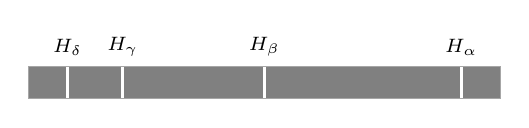
\begin{tikzpicture}[font=\scriptsize]
	\draw[fill=gray,draw=gray!70] (0,0) rectangle(6,.4);
	\draw[draw=white,very thick] (.5,0)--(.5,.4)node[above]{\(H_{\delta}\)} (1.2,0)--(1.2,.4)node[above]{\(H_{\gamma}\)} (3,0)--(3,.4)node[above]{\(H_{\beta}\)} (5.5,0)--(5.5,.4)node[above]{\(H_{\alpha}\)};
\end{tikzpicture}
\begin{choices}
	\item 照射同一单缝衍射装置，\(H_{\delta}\)光的中央明条纹宽度宽		
	\item 以相同的入射角斜射入同一平行玻璃砖，\(H_{\delta}\)光	的侧移量小
	\item 以相同功率发射的细光束，真空中单位长度上
		\(H_{\gamma}\)光的平均光子数多
	\item 相同光强的光分别照射同一光电效应装置，\(H_{\gamma}\)	光的饱和光电流小
\end{choices}
\begin{answer}
    
\end{answer}